\section{\review{Summary}}

% Intro, Chromatic AmpDet & Decay
The corrections of third order chromaticity $Q'''$ has been observed in the past to show
discrepancies to the magnetic model at injection energy, prompting an investigation of the decapolar
errors using various observables to identify their sources. To better understand these
discrepancies, novel observables such as bare chromaticity and chromatic amplitude detuning were
introduced.
%
Chromatic amplitude detuning, which accounts for the detuning via both horizontal and vertical
actions with to momentum offset, differs in expression from standard chromaticity and provides a
more comprehensive view of decapolar errors. This observable was measured for the first time at the
LHC.
%
Simulations suggest that the decay of the decapolar component in the main dipoles is the major
factor contributing to these discrepancies. This component had previously been neglected in both
beam dynamics studies and operational correction strategies.

% RDT
For the first time, measurements and direct corrections of the decapolar Resonance
Driving Term (RDT) $f_{1004}$ were carried out. Further simulations and measurements explored how
sextupoles and octupoles interact to create decapolar-like fields. The findings revealed that
sextupoles, both alone and in combination with Landau octupoles, generate substantial decapolar RDTs
via feed-up during machine operation that could benefit from corrections.


% Impact
Applying combined corrections for third-order chromaticity, chromatic amplitude detuning, and the
RDT $f_{1004}$ led to a $3\%$ improvement in beam lifetime. Additionally, a broader impact of
decapolar RDTs on beam stability was investigated. Specifically, intentionally degrading the RDT
$f_{1004}$ resulted in a decrease in beam lifetime of about $10\%$. 
Furthermore, a significant improvement in the forced dynamic aperture during AC-Dipole excitation
was observed when corrections were applied. The earlier corrections for decapolar errors were
implemented alongside octupolar corrections for $Q''$. \Cref{fig:decapoles:losses_b4b5_corrs}
demonstrates the relative losses encountered when kicking at different amplitudes with the
AC-Dipole. This clearly shows that octupolar and decapolar corrections enhance the forced dynamic
aperture.

\begin{figure}[!htb]
    \centering
    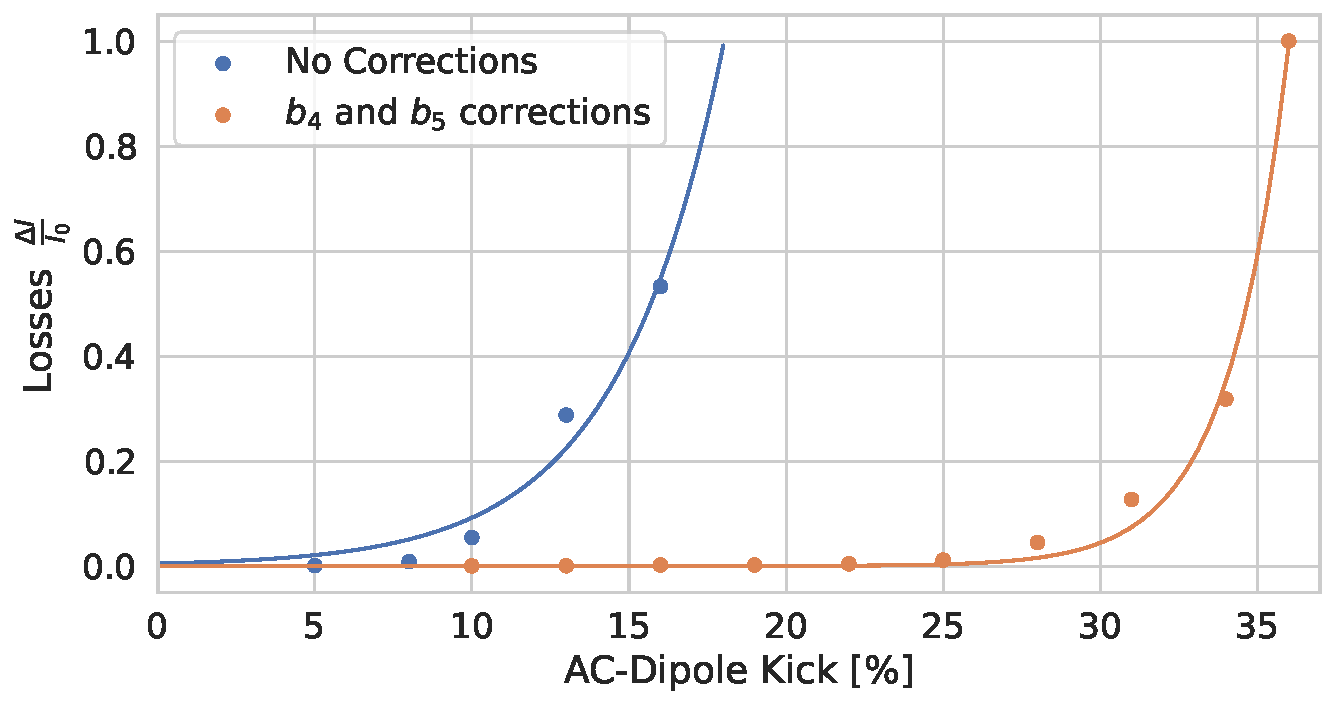
\includegraphics[width=0.8\textwidth]{./images/losses_with_without_b4b5corr.pdf}
    \caption{Relative losses experienced with AC-Dipole kick amplitude with and without corrections
    pertaining to $Q''$, $Q'''$, chromatic amplitude detuning, and RDT $f_{1004}$.}
    \label{fig:decapoles:losses_b4b5_corrs}
\end{figure}

% Corrections implemented and outlook
Initially, the feed-up effect was not well understood, leading to the decision to exclude any
decapolar corrections from the machine. However, through studies of decapolar perturbations and the
interaction of various multipoles, significant progress was made. The magnetic model for $b_5$
errors is now more complete, enabling the implementation of these corrections in the machine, which
has resulted in both increased lifetime and the possibility of higher-amplitude kicks for non-linear
optics studies.
%
Advancements in understanding the magnetic model and controlling decapolar errors are crucial not
only for the HL-LHC but also for the FCC-ee, which will depend on precise control of $b_5$ errors to
optimize dynamic aperture.